\part{A - Main}
\section{Introduction}

\begin{frame}{Conflicts in Real Life}
\vspace{-0.5cm}
\begin{center}
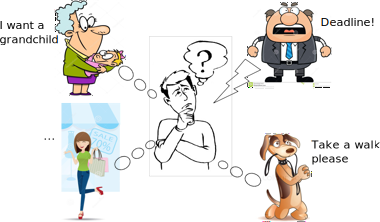
\includegraphics[width=0.88\textwidth]{conflict-real-life}
\end{center}
\end{frame}


\begin{frame}{Conflicts in SDN}
\advance\leftskip+1cm\includegraphics<1>[width=0.8\textwidth]{conflict-sdn1}
\includegraphics<2>[width=0.8\textwidth]{conflict-sdn2}
\includegraphics<3>[width=0.8\textwidth]{conflict-sdn3}

\begin{onlyenv}<4>
\begin{columns}[c]
\column{0.1\textwidth}
\column{0.5\textwidth}
\vspace{1cm}

\textbf{Possible consequences:} 
\begin{itemize}
\item Application's goals are not fulfilled
\item Unexpected, unreliable network behaviour
\end{itemize}
$\textcolor{lmu@hyperlink}{\Rightarrow}$ Conflicts need to be detected and resolved
\column{0.5\textwidth}
\vspace{1cm}
\noindent
\includegraphics[width=\textwidth]{conflict-sdn3}
\column{0.2\textwidth}
\end{columns}
\end{onlyenv}
\end{frame}


\begin{frame}{Conflict Definition}
\vspace{0.5cm}
\begin{center}
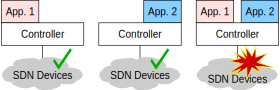
\includegraphics[width=0.7\textwidth]{conflict-definition}
\end{center}
\end{frame}


%\begin{frame}{Goal}
% Goal of this work
%\end{frame}


\begin{frame}{Research Questions}
\vspace{-0.2cm}
\begin{enumerate}
\item<1-> What is a suitable method to research conflicts in SDN? 
\item<1-> How can conflicts between control applications be classified\\ based on their rules (conflict classification)? 
\item<2-> How many conflicts exist in a given rule set (conflict detection)?
\begin{enumerate}
\item Which rules cause conflicts?
\item To which class does each detected conflict belong?
\end{enumerate}

\vspace{0.4cm}

\advance\leftskip+0.7cm
\includegraphics<2>[height=0.45\textheight]{cdinout_highlighted}
\includegraphics<3>[height=0.45\textheight]{cdinout_highlighted_next}
\end{enumerate}

\end{frame}


\section{Related Work}

\begin{frame}{State-of-the-art}
\begin{itemize}
\item Related work 1
\item Related work 2
\item \ldots
\end{itemize}
\end{frame}


\section{Approach}

\begin{frame}{Approach}
\begin{enumerate}
\item Analytical approach 
\item Experimental approach
\end{enumerate}
\end{frame}


\subsection{Experimental approach}

\begin{frame}{Space for Experiments}

\begin{columns}[T]
\column{0.6\textwidth}
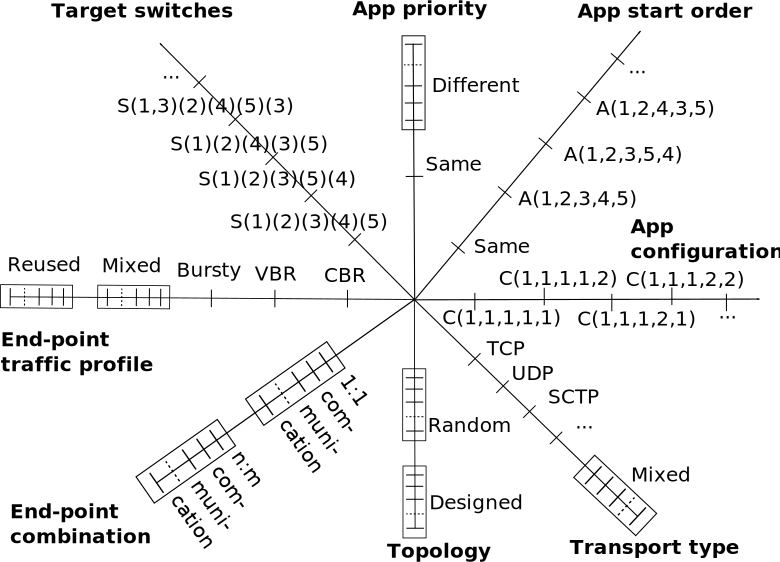
\includegraphics[width=\textwidth]{parameter-space}

\column{0.45\textwidth}
\vspace{7ex}

\begin{onlyenv}<1>
Control applications: 
\begin{itemize}
\item Shortest Path First Routing (SPF)
\item End-point Load Balancer (EpLB)
\item Path Load Balancer (PLB)
\item Firewall (FW)
\item \ldots
\end{itemize}
\end{onlyenv}
\begin{onlyenv}<2>
The number of experiments is immense \\[8pt]
$\textcolor{lmu@hyperlink}{\Rightarrow}$ \textbf{restrict the space size and automate experiments}
\end{onlyenv}
\end{columns}
\end{frame}

\subsection{Methodology for experiments}

\begin{frame}{Methodology for Experiments}
\vspace{-0.3cm}
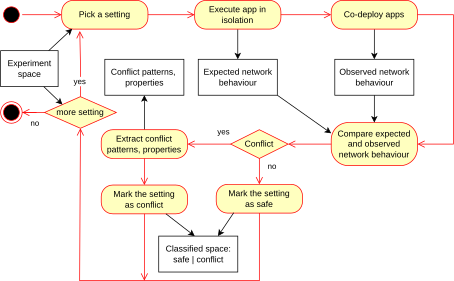
\includegraphics[height=\textheight]{methodology-exp}
\end{frame}


\subsection{Explored subspaces}

\begin{frame}{Explored Subspaces}
\begin{columns}[T]
\column{0.05\textwidth}
\column{0.5\textwidth}
\vspace{0.2cm}
\begin{tabular}{|l|c|}
%\hline
%\textbf{Category} & \textbf{Value} \\
\hline
\# Topologies & 12 \\
\hline
\# Applications & 14  \\
\hline
App. configuration & 1 $\rightarrow$ 5  \\
\hline
App. start order & same and different \\
\hline
App. priority & same and different \\
\hline
Target switches & 1 $\rightarrow$ all \\
\hline
Ep. Traffic Profile & CBR and VBR  \\
\hline
EP. Combination & unicast, multicast \\
\hline
Transport type & TCP, UDP  \\
\hline
\# Experiments & 11,772 \\
\hline
\end{tabular}

\column{0.5\textwidth}
\vspace{0.5cm}
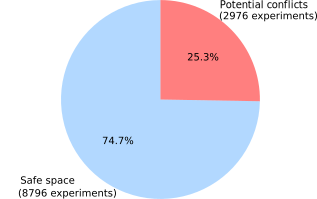
\includegraphics[width=\textwidth]{pie_exp}
\column{0.05\textwidth}
\end{columns}
\vspace{0.3cm}
\scriptsize{Dataset is available at \\https://github.com/mnm-team/sdn-conflicts}
\end{frame}


\section{Multi-property set}

\begin{frame}{Comparing Multi-Property Sets using $\cdot r$}
\vspace{-0.3cm}
\advance\leftskip+1cm 
\includegraphics<1>[height=\textheight]{multi_property_set_comparison_1}
\includegraphics<2>[height=\textheight]{multi_property_set_comparison_2}
\includegraphics<3>[height=\textheight]{multi_property_set_comparison_3}
\includegraphics<4>[height=\textheight]{multi_property_set_comparison_4}
\end{frame}


\section{Prototype}

\begin{frame}{Conflict Detection Prototype}
\vspace{-0.3cm}
\advance\leftskip+1.5cm 
\includegraphics<1>[height=\textheight]{cd_communication}
\includegraphics<2>[height=\textheight]{cd_communication_zoom}
\end{frame}


\section{Evaluation}

\begin{frame}{Detected Results in Designed Cases}

Rules are deployed with known conflicts

Conflicts detected by the prototype are then controlled manually\\[12pt]

Results for both MWN and Stanford topologies:\\[4pt]

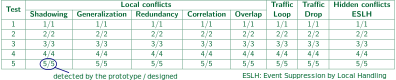
\includegraphics[width=1.05\textwidth]{evares-designed}

\vspace{0.3cm}

$\textcolor{lmu@hyperlink}{\Rightarrow}$ All conflicts are precisely identified

\end{frame}


\section{Conclusions}

\begin{frame}{Conclusions}
\vspace{-0.3cm}
\includegraphics<1>[height=\textheight]{conclusion_rq} %research questions
\includegraphics<2>[height=\textheight]{conclusion}
\end{frame}


\section{Prospects}

\begin{frame}{Prospects}
\vspace{0.3cm}

\begin{itemize}
\item Future work 1
\item Future work 2
\item \ldots
\end{itemize}
\end{frame}
